\documentclass[A4s]{beamer}
\usetheme{MASL}
\usepackage[orientation=landscape,size=a1,scale=1.1,debug]{beamerposter}
\usepackage{etex}
\usepackage[absolute,overlay]{textpos}
\setlength{\TPHorizModule}{1cm}
\setlength{\TPVertModule}{1cm}

\newcommand{\bX}{\textbf{X}}

\usepackage{graphicx}
\usepackage{wrapfig}
\usepackage{graphicx}
\usepackage{xcolor}
\usepackage{pstricks}
\usepackage{tikz}
\usepackage{listings}
\usepackage{tcolorbox}

\definecolor{gray}{rgb}{.6,.6,.6}
\definecolor{orange}{rgb}{1,0.5,0}
\definecolor{grayish}{rgb}{.9, .9, .9}
\definecolor{dkgray}{rgb}{.375, .375, .375}
\definecolor{dkgreen}{rgb}{0,0.6,0}
\definecolor{mauve}{rgb}{0.58,0,0.82}
\definecolor{dkblue}{rgb}{0, 0, .5}

\lstset{ %
  language=R,    
  numbers=left,
  stepnumber=1,       
  numbersep=6pt,      
  showspaces=false,      
  showstringspaces=false,  
  showtabs=false,    
  frame=single,      
  rulecolor=\color{black},   
  tabsize=4,     
  captionpos=t,     
  breaklines=true,     
  breakatwhitespace=true,   
  title=\lstname,              
  basicstyle=\ttfamily\color{black}\scriptsize, 
  backgroundcolor=\color{grayish},  
  numberstyle=\tiny\color{black},  
  keywordstyle=\color{blue}, 
  commentstyle=\color{dkgreen}, 
  stringstyle=\color{mauve}, 
  xleftmargin=.3in,
  xrightmargin=.3in,
  aboveskip=-0.8cm,
  belowskip=.2cm,
  morekeywords={expm, ddmatrix}
}



  

\def\mytemparray{}

\newcommand\doatpos[3]{%
    \bgroup
    \def\mytemparray{{ #2 }}
    \pgfmathparse{\mytemparray[0]} \edef\mya{\pgfmathresult}
    \pgfmathparse{\mytemparray[1]} \edef\myb{\pgfmathresult}
    \pgfmathparse{\mytemparray[2]} \edef\myc{\pgfmathresult}
    \begin{tikzpicture}[remember picture, overlay]
      \node[anchor=#1, opacity=\myc] at ( \mya pt, \myb  pt) {#3};
    \end{tikzpicture}%
    \egroup
}
\usepackage{caption}
\usepackage{subcaption}


\newcommand{\pulltotop}{\ \vspace{-7.4cm}}


\title{XSEDE Text Analytics Gateway}
\author{Mike Black$^1$ and Drew Schmidt$^2$\\[.2cm]
  $^1$University of Illinois, $^2$University of Tennessee\vspace{-.2cm}}
\date{}

\footer{\makebox[.975\paperwidth]{%
  
\includegraphics{pics/xsede_small}
  \hfill%
  \small \url{https://github.com/XSEDEScienceGateways/TAG}\hspace{0ex}%
%   \rput[b]{20}(-.35,-.8){
\includegraphics[scale=.42]{pics/qr_tag_github}}%
}}



\begin{document}

\begin{frame}[fragile]{} 
\begin{pspicture}(3,-30)(\linewidth,0)
\doatpos{west}{.9cm, 11.9cm, .5}%
{
\includegraphics[scale=.39]{./pics/utk}}
\doatpos{west}{77.75cm, 11.92cm,.5}%
{
\includegraphics[scale=.75]{./pics/uiuc}}

 
 

\begin{columns}[T]
\hspace{.3cm}



%%%%%%%%%%%%%%%%%%%%%%%%%%%%%%%%%%%%%%%%%%%%%%%%%%%%%%%%%%%%%%%%%%%%%%%%%%%%%%%%
%%%%%%%%%%%%%%%%%%%%%%%%%%%%%%%%%%%%%%%%%%%%%%%%%%%%%%%%%%%%%%%%%%%%%%%%%%%%%%%%
%%%%%%%%%%%%%%%%%%%%%%%%%%%%%%%%%%%%%%%%%%%%%%%%%%%%%%%%%%%%%%%%%%%%%%%%%%%%%%%%
\begin{column}{.31\paperwidth}
\pulltotop


\begin{block}{Background}
\begin{itemize}
  \item Humanities and social sciences historically dominated by qualitative 
methods.
  \item Researchers in these fields increasingly turning to quantitative methods 
and computational resources to answer larger questions.
  \item Still much resistance, often driven by a ``technological 
familiarity gap''.
\end{itemize}
\vspace{.8cm}

So why expect users to start with this?

\begin{lstlisting}[language=R]
corpus <- tm::tm_map(corpus, tm::content_transformer(base::tolower))
corpus <- tm::tm_map(corpus, tm::removePunctuation)
corpus <- tm::tm_map(corpus, tm::removeNumbers)
corpus <- tm::tm_map(corpus, tm::stripWhitespace)
corpus <- tm::tm_map(corpus, tm::removeWords, 
    tm::stopwords(input$data_filter_stopwords_lang))
tdm <- tm::TermDocumentMatrix(corpus)
wordcount_table <- sort(rowSums(as.matrix(tdm)), decreasing = TRUE)
\end{lstlisting}
\vspace{.8cm}

Programming is great!  But...
\begin{itemize}
  \item Users often lack the background and have little access to training.
  \item No institutional rewards for developing technical skills.
  \item Programming vs GUI:  Recall vs. recognition.
\end{itemize}

\end{block}


\begin{block}{TAG: The Text Analytics Gateway}
  \begin{center}
    Basic Text Analysis Tools Without the Programming
  \end{center}

  \begin{minipage}[t]{.5\textwidth}
    \begin{center}
    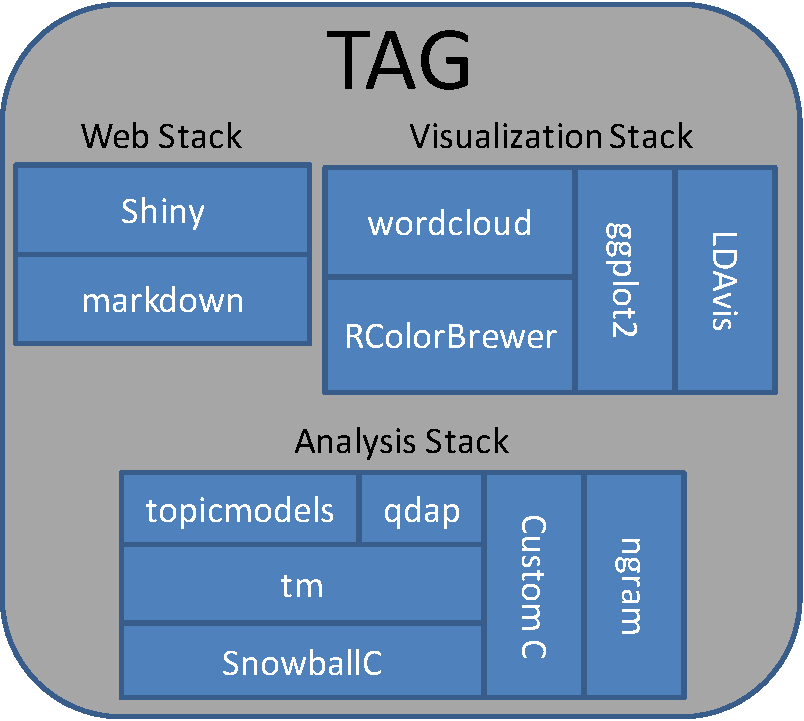
\includegraphics{pics/tag}
  \end{center}
  \end{minipage} \quad
  \begin{minipage}[t]{.42\textwidth}
  \vspace{.6cm}
    \begin{itemize}
      \item Written mostly in R.
      \item Extensive re-use of existing R packages.
      \item UI served via shiny~\cite{shiny} and shiny server.
      \item Some custom high-performance C.
      \item Help files written in markdown, rendered on the fly.
    \end{itemize}
  \end{minipage}
  \vspace{.8cm}
  
  Offer full analysis pipeline, by combining:\\\vspace{-.5cm}
  \begin{minipage}[t]{.45\textwidth}
    \begin{itemize}
      \item Data retrieval
      \item Preprocessing
    \end{itemize}
  \end{minipage}
  \quad
  \begin{minipage}[t]{.45\textwidth}
    \begin{itemize}
      \item Data retrieval
      \item Preprocessing
    \end{itemize}
  \end{minipage}
  \vspace{.4cm}
  
  into a single, complete workflow.
\end{block}




\end{column}



%%%%%%%%%%%%%%%%%%%%%%%%%%%%%%%%%%%%%%%%%%%%%%%%%%%%%%%%%%%%%%%%%%%%%%%%%%%%%%%%
%%%%%%%%%%%%%%%%%%%%%%%%%%%%%%%%%%%%%%%%%%%%%%%%%%%%%%%%%%%%%%%%%%%%%%%%%%%%%%%%
%%%%%%%%%%%%%%%%%%%%%%%%%%%%%%%%%%%%%%%%%%%%%%%%%%%%%%%%%%%%%%%%%%%%%%%%%%%%%%%%
\begin{column}{.31\paperwidth}
\pulltotop


\begin{block}{TAG Features}
  Detailed summary statistics 
  \begin{center}
    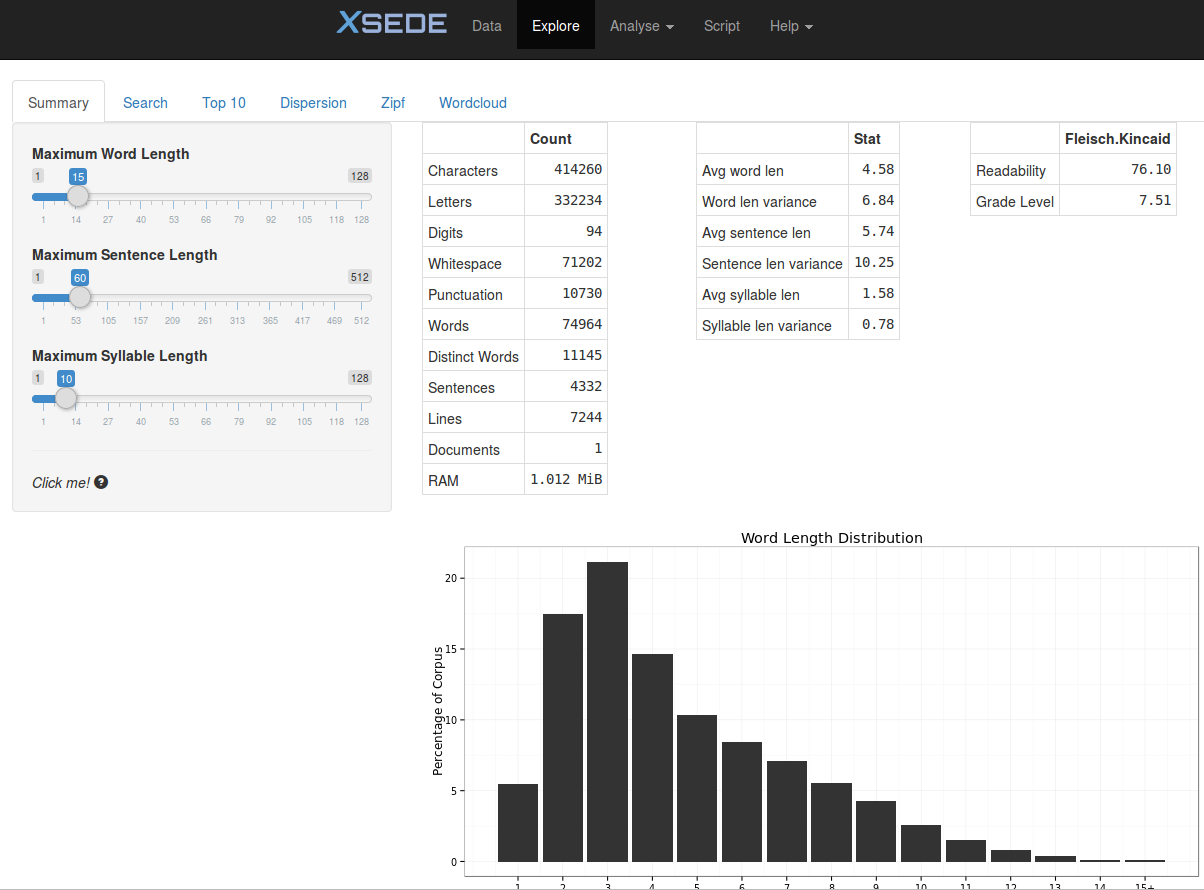
\includegraphics[width=.9\textwidth]{pics/explore}
  \end{center}
  
  Includes LDAvis~\cite{ldavis} for powerful topic modeling visualization:
  \begin{center}
    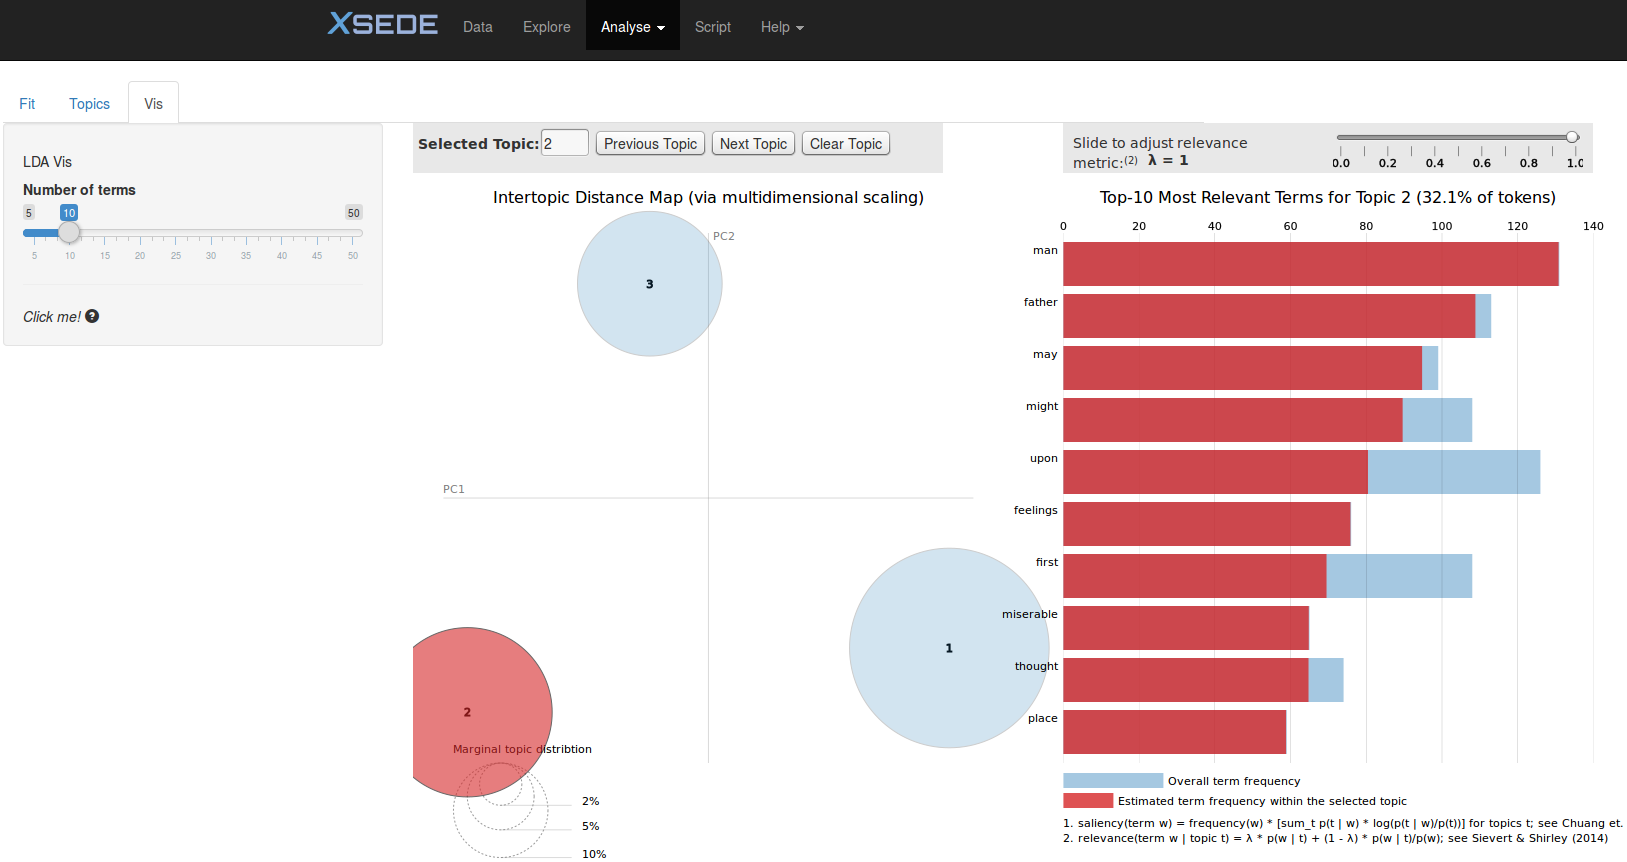
\includegraphics[width=.9\textwidth]{pics/ldavis}
  \end{center}
  
  And more\dots
    \begin{itemize}
    \item \textbf{Processing:} Text filtering and transformations.
    \item \textbf{Vis:} Dispersion plots and wordclouds.
    \item \textbf{Analysis:}  LDA and n-gram modeling.
    \item \textbf{Reproducibility:} State management, script generation.
  \end{itemize}
\end{block}

\end{column}



%%%%%%%%%%%%%%%%%%%%%%%%%%%%%%%%%%%%%%%%%%%%%%%%%%%%%%%%%%%%%%%%%%%%%%%%%%%%%%%%
%%%%%%%%%%%%%%%%%%%%%%%%%%%%%%%%%%%%%%%%%%%%%%%%%%%%%%%%%%%%%%%%%%%%%%%%%%%%%%%%
%%%%%%%%%%%%%%%%%%%%%%%%%%%%%%%%%%%%%%%%%%%%%%%%%%%%%%%%%%%%%%%%%%%%%%%%%%%%%%%%
\begin{column}{.31\paperwidth}
\pulltotop

\begin{block}{Timeline and Status}
  \begin{itemize}
    \item November 12, 2014:  Allocation awarded.
    \item April 6, 2015:  PI connected to ECSS staff.
    \item April 6---March 15, 2015:  Research technology stack.
    \item Mar 20, 2015:  Development begins.
    \item July 7, 2015:  Gateway stood up on AWS. Usability studies begin.
    \item Soon:  live on Comet, tutorials, workshops\dots
  \end{itemize}
  
  \begin{figure}
    \centering
    \begin{subfigure}[b]{0.4\textwidth} 
      \centering
      
\includegraphics[width=\textwidth]{pics/comet}
      \caption{Coming soon\textsuperscript{TM} to Comet!} 
    \end{subfigure} ~ 
    \begin{subfigure}[b]{0.4\textwidth}
      \centering
      
\includegraphics[width=.7\textwidth]{pics/qr_tag_live}
      \caption{Try now on our AWS hosting!} 
    \end{subfigure}
    \end{figure}
\end{block}


\begin{block}{Future Work}
  \begin{itemize}
    \item Stand up gateway on Comet.
    \item Incorporate multidocument support.
    \item Add sentiment analysis feature.
    \item Develop userbase and community.
  \end{itemize}
\end{block}


\begin{block}{References}
\begin{thebibliography}{}
\setbeamertemplate{bibliography item}[text]
\setbeamercolor{bibliography item}{fg=black}
\setbeamercolor*{bibliography entry title}{fg=black}

    \bibitem{shiny}
    {Winston Chang, Joe Cheng, JJ Allaire, Yihui Xie and Jonathan
  McPherson (2015). shiny: Web Application Framework for R. R package
  version 0.12.1.9000. http://shiny.rstudio.com}
    
    \bibitem{ldavis}
    {Carson Sievert and Kenny Shirley. LDAvis: Interactive
  Visualization of Topic Models. R package version 0.3.1.
  https://github.com/cpsievert/LDAvis}
\end{thebibliography}
\end{block}

\begin{block}{Acknowledgements}
  This work used the Extreme Science and Engineering Discovery Environment 
(XSEDE), which is supported by National Science Foundation grant number 
OCI-1053575 and the XSEDE Science Gateways Program.
\end{block}



\end{column}
%%%%%%%%%%%%%%%%%%%%%%%%%%%%%%%%%%%%%%%%%%%%%%%%%%%%%%%%%%%%%%%%%%%%%%%%%%%%%%%%%%%%
%%%%%%%%%%%%%%%%%%%%%%%%%%%%%%%%%%%%%%%%%%%%%%%%%%%%%%%%%%%%%%%%%%%%%%%%%%%%%%%%%%%%
%%%%%%%%%%%%%%%%%%%%%%%%%%%%%%%%%%%%%%%%%%%%%%%%%%%%%%%%%%%%%%%%%%%%%%%%%%%%%%%%%%%%

\end{columns}

\doatpos{west}{-47.015cm, -39.7cm,.5}{
  
\includegraphics[scale=1.045]{pics/tag_small}%
}

\end{pspicture}

\end{frame}
\end{document}
